\section{Extract the List}
\label{sec:extractList}

If a web page contains a ``top-$k$ like'', our system will look into the body of the page to find a list of $k$ items.
which are text nodes generally.
\footnote{Although we are also interested in images (nodes with tag {\tt <img>}) and table cells (nodes with tag{\tt <td>}), we convert them into text nodes with special format and handle them with the same method as the normal text nodes}
As we mentioned before, we can do this through first collecting a set of candidate lists by the candidate picker, and then selecting the best one as result by the ``top-$k$'' ranker.
If we can successfully get such a list, we will make some postprocessing to the list in the content processor.
Otherwise, we will declare that the page does not contain a ``top-$k$'' list and therefore is not a ``top-$k$'' page.

In Section \ref{sec:evalList}, we test the performance of this part solely. In order to avoid the effect of the title classifier. We use a set of 100 real ``top-$k$'' pages. The experimental result is shown in Table\ref{tab:listRes}, which presents very good performance in both precision and recall.

\subsection{Prepare the DOM Tree}
Since the input is raw HTML text, we need to parse it into a DOM tree first.
In our system, we use Winista HtmlParser \cite{winista}.
After parsing, the parser will return a node which is the root node of the DOM tree.
To analyze the tree, we can recursively traverse the tree from the root node.

In order to make the tree representation clear and normalized, we preprocess all the tree nodes in the following several aspects.

\begin{itemize}
  \item \textbf{Filter unwanted nodes}:
  As we mentioned in Section \ref{sec:DOMtree}, we will remove all the comment nodes in the DOM tree since they are nothing to do with the actual page rendering. In addition, we keep a black list of tags which are unlikely to contain a ``top-$k$'' list. We list those tag names in Table \ref{tab:blackTag}.
  \item \textbf{Combine adjacent siblings}:
  In some cases, two adjacent tag nodes may be of the same tag name. For some particular tags, such as {\tt <strong>} and {\tt <i>} we can move the the child nodes of the latter node into the former and remove the latter node, i.e., combine the two nodes together. This replacement will not affect the display effect and make the tree clearer. However this does not work for all the tags, for example, if we combine two adjacent ``h1'' tags, the rendering of the page will be changed.
  \item \textbf{Handle image tags}:
  Our system is originally designed to extract text node lists.
  Later we find that images are also useful to describe list items, for example the third column in Table \ref{tab:sampleoutput}.
  In order to make the system compatible to image tag nodes, we can replace a image node with a text node, the content of which is specified by the image URL. Therefore, we can extract image lists just like other normal lists and then retrieve the images by the URLs.
\end{itemize}

\begin{table}
\centering
\caption{The black list of tag name}
$
\begin{array}{|cccccc|}
\hline
  head & link & style & form & iframe & input \\
\hline
\end{array}
$

\label{tab:blackTag}
\end{table}


\subsection{Collect Candidates}
\label{sec:picker}
Given an HTML page body and the number $k$,
the candidate picker collects a set of lists as candidates.
Each list item is a text node in the page body.

%We define a {\em tag path} of a node as a path from the root to this node
%in the DOM tree.
Items in a ``top-$k$'' list usually have similar format and style,
and therefore they share an identical tag path.
For example, in Table \ref{tab:sampleoutput},
the tag path corresponding to the second column {\em Name} is
{\tt html/body/.../p/strong}.

Based on this observation, our algorithm runs in following steps:

\begin{enumerate}
  \item \textbf{Compute the tag path for each node}:
  We can recursively traverse the DOM tree and get the tag paths for all nodes.
  The tag path of a node $n$ can be calculated by the following equation:
  \begin{equation}\label{equ:tagPath}
    n.TagPath=n.Parent.TagPath+Splitter+n.TagName;
  \end{equation}
  In this equation, the splitter is a constant string which serves as boundaries between tag names in the tag path.
  Since the values in Equation \ref{equ:tagPath} are all strings,
  the plus sign means to concatenate the strings of both sides.
  In addition, as is suggested by Equation \ref{equ:tagPath}, we should know the tag path of the parent node in advance.
  Therefore, the traversal is done in a preorder manner.

  \item \textbf{Group text nodes with an identical tag path}:
  After computing the tag path we have a mapping from a node to a tag path string. Then we want the reverse mapping,
  which is from a tag path to a list of nodes that share the tag path. We can use a hash table as the data structure, of which the key type is string and value type is list of node.
  We can traverse all the text nodes and for each node $n$,
  we insert itself to the node list that is corresponding to $n$'s tag path in the hash table
  (if the table does not contain $n$'s tag path as key yet, insert the tag path with a value of a new empty list into the table).

  \item \textbf{Select $k$-item lists}:
  With a table of node lists of equivalent tag paths(as keys), we select those node lists of $k$ items (i.e, $k$ text nodes).
  We consider them as candidate lists.
\end{enumerate}

In our implementation, we put the first and second step together in one traversal, which is shown in Algorithm \ref{algo:tagPaht} 
(see \ref{appendix:algo}).

%Algorithm \ref{algo:tagPaht} just shows a general idea which ignores some optimizations in this part.
%TODO


%Based on this observation, our algorithm runs in four steps:
%First, we preprocess the DOM tree to normalize the content of text nodes
%(remove non-printable characters and shorten continuous spaces, etc.).
%Second, we prune the DOM tree by cutting subtrees that include ``blacklisted''
%attributes such as ``sidebar'' and ``comment'', because these often indicate
%they are not the main content of the page.
%so that we can get avoid of most adversitements and user comments.
%Third, we compute the tag path for every node in the DOM tree of the
%input page. Finally, we group nodes with an identical tag path into
%one {\em equivalence class}, and we
%select those equivalence classes which have exactly $k$ members as our
%candidate lists.

Algorithm \ref{algo:tagPaht}, known as the {\em Default} algorithm, achieves good
recall, but may produce noise. To further improve the precision,
we introduce three additional pattern-based rules to filter the candidate lists:

\begin{enumerate}
\item \textit{Index}:
There exists an integer number in front of every list item, serving as
a rank or index: e.g., ``1.'',``2.'',``3.'', ..., the numbers are in sequence
and within the range of $[1, k]$ (e.g., Figure \ref{fig:indexPattern}).

\item \textit{Highlighting tag}:
The tag path of the candidate list contains at least one tag
among {\em <b>,<strong>,<h1-h6>} for highlighting purposes(e.g., Figure \ref{fig:highlightPattern}).

\item \textit{Table}:
The candidate list is shown in a table format(e.g., Figure \ref{fig:tablePattern}).
\end{enumerate}

\begin{figure}[th]
\centering
\epsfig{file=pics/indexPattern.eps,width=0.6\columnwidth}
\caption{A sample list of index pattern\cite{Top20Books}}
\label{fig:indexPattern}
\end{figure}

\begin{figure}[th]
\centering
\epsfig{file=pics/highlightPattern.eps,width=1.0\columnwidth}
\caption{A sample list of highlight pattern\cite{highlightPattern}}
\label{fig:highlightPattern}
\end{figure}

\begin{figure}[th]
\centering
\epsfig{file=pics/tablePattern.eps,width=0.7\columnwidth}
\caption{A sample list of table pattern\cite{tablePattern}}
\label{fig:tablePattern}
\end{figure}

In this modified algorithm, a.k.a. {\em Def+Patt} algorithm,
only candidates that satisfy at least one of the rules above are
kept and output to the next step.
For example the ``top-$k$'' list in Figure \ref{fig:topscientists}
satisfies Rule 1 and 2.

\subsection{Rank and Select the Top-K List}
\label{sec:ranker}

When there are multiple candidate lists,
we select only one of them as the {\em main list}.
We can rank each candidate list with a score, the one with highest score will be selected as the result.
To calculate the score, we set a few criteria as follows:

\begin{itemize}
  \item \textbf{$P\textnormal{-}Score$}:

  $P\textnormal{-}Score$ is to measure the correlation between the list and title.

  Intuitively, the main list is the one that best matches the title.
In Subsection \ref{sec:title}, we extract a set of concepts from
the title, and one of them should be the central concept of the ``top-$k$'' list.
Our key idea is that one or more items from the main list should be instances
of one of the concepts extracted from the title. For example, if the title
contains the concept ``scientist'', then the items of the main list should
be {\em instances} of the ``scientist'' concept. The Probase taxonomy provides
large number of concepts and their instances which were extracted from the
web corpus. For instance, ``scientist'' concept has 2054 instances in
Probase.

We calculate the $P\textnormal{-}Score$ of each candidate list $L$ as:

\begin{equation}\label{equ:pScore}
    P\textnormal{-}Score= \frac{1}{k} \sum_{n \in L} \frac{LMI(n)}{Len(n)};
\end{equation}
where $LMI(n)$ is the word count of the longest matched
instance in the text of node $n$,
while $Len(n)$ means the word count of the whole text in node $n$.

Form Equation we can see that, the $P\textnormal{-}Score$ of a list is the average of the ``$P\textnormal{-}Score$'' ($\frac{LMI(n)}{Len(n)}$) of each node.
The reason to divide $LMI(n)$ with $Len(n)$ is that we therefore can normalize P-Score to the range $[0,1]$, and the contribution of each node will be no more than $1/k$, which make sure that one single node cannot affect the whole $P\textnormal{-}Score$ too much. In addition, we want $P\textnormal{-}Score$ to prefer to lists with fewer words, since nodes with many words(like description) are more likely to have a higher $LMI$.

  \item \textbf{$V\textnormal{-}Score$}:

$V\textnormal{-}Score$ calculates the visual area occupied by a list,
since it is also reasonable for the main list of the page to be larger and more attractive than other minor lists.

The $V\textnormal{-}Score$ of a list is the sum of the visual area of each node.
The visual area is estimated by calculating text area
of the candidate list:

\begin{equation}\label{equ:vScore}
Area(L)= \sum_{n \in L} (TextLength(n)\times FontSize(n)^2).
\end{equation}

  \item \textbf{$Bonus$}:

  With $bonus$, we can import heuristic rules to the ranking system. Note that bonus can also be negative, which is actually penalty.

  For example, we want to show priorities to the lists that matches the three patterns(index, highlight and table), so we give them a large positive bonus. On the contrary, nodes in some list contain negative attribute values such as ``sidebar'' or ``comment'',
  which imply the list a non-``top-$k$'' list. We should assign them a negative bonus.

\end{itemize}

The final score $F\textnormal{-}Score$ can be calculated by Equation \ref{equ:fScore}:

\begin{equation}\label{equ:fScore}
    F\textnormal{-}Score(L)= \lambda F\textnormal{-}Score(L)+ \mu V\textnormal{-}Score(L)+Bonus(L);
\end{equation}

where $\lambda$ and $\mu$ are weights for each score, which are determined by experimental experiences
($\lambda=0.7, \mu=0.3$ in our system).

After we know the main list, we can also get attribute lists to form a table like Table \ref{tab:sampleoutput}.
The attribute lists should also be candidate lists and they should be interleaved with the main list.

\subsection{Prepare the result}

Hopefully, we can extract a raw ``top-$k$'' list after previous steps. And now in the concept processor,
we would like to further process the content of list items to make the result cleaner and more meaningful.

For example, the content processor can transfer the raw list in Table \ref{tab:rawList} into Table \ref{tab:processedList}.
In the latter table, there are mainly two improvements: first, we move the content in the bracket to a new column; second, we create a table head and conceptualize each column.

Generally, the content processor has two tasks:

\begin{itemize}
  \item \textbf{Infer the inner structure}:

  In some cases, the text node of the raw list may have some inner structure itself. For example, the inner structure of the list in Table \ref{tab:rawList} is ``XXXX(YYYY)''. The inner structure enables the text node to contain multiple kinds of information, which should be explicitly divide into fields.

  The content processor infers the structure of
the text \cite{Fisher08:dirttoshovels} by building a histogram for
all potential separator tokens such as ``By'', ``:'' and ``,'' from all the items
of the ``top-$k$'' list.
The x-axis represents the occurrence number of a separator in a node,
while the y-axis means the number of nodes.
If we identify a sharp spike in the histogram for a
particular token, which means the occurrence number of the separator is identical among all the list nodes, then we successfully find a separator token, and we use that
token to separate the text into multiple fields.
Figure \ref{fig:histogram} presents the histogram for the list in Table \ref{tab:rawList}, we can clearly see that the separator bracket has a sharp spike which other separators (dot and comma) do not have.

  \item \textbf{Conceptualize the list}:

  It is useful provide names to the extracted attribute values. For example,
we want to infer ``image'', and ``Wikipedia link'' as
attribute names from the list in Figure \ref{fig:topscientists}.
To do this, we conceptualize the extracted columns \cite{Song11:Conceptualize},
using Probase and a Bayesian model,
which we have made a brief introduction in Section \ref{sec:shortText}.
We can use the longest instance to represent the observed instance of each node in the list, thus we can get an instance set $E=\{e_{i},i \in 1,...,k\}$. Apply $E$ to Equation \ref{equ:shortText1} then we can get the conditional probability of concepts.
The concept with the max probability will be selected to conceptualize the list.
In addition, for special columns like indexes, pictures and long paragraphs,
we apply specified rules to conceptualize them.

\end{itemize}

\begin{figure}[th]
\centering
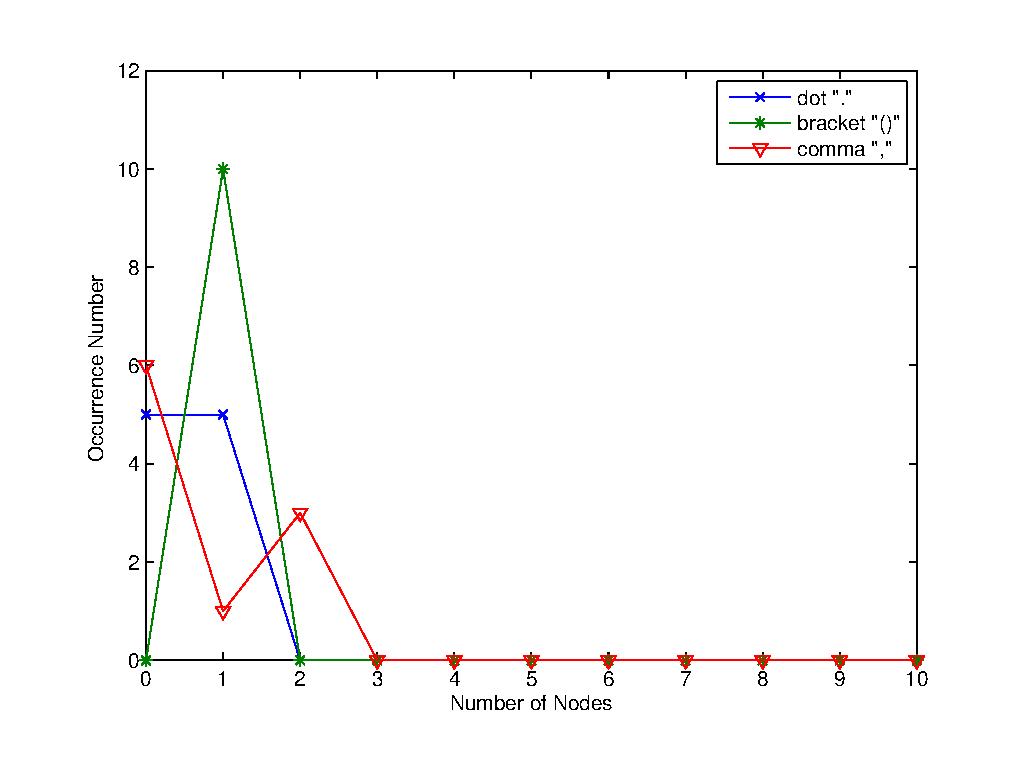
\epsfig{file=pics/histogram.eps,width=0.9\columnwidth}
\caption{The histogram for the list in Table \ref{tab:rawList}}
\label{fig:histogram}
\end{figure}

\begin{table}
\centering
\caption{The raw result of a ``top-$k$'' list fragment\cite{top100Newspapers}}
\begin{tabular}{|l|}
\hline
USA Today (Arlington, Va.)\\
Wall Street Journal (New York, N.Y.)\\
Times (New York, N.Y.)\\
Times (Los Angeles)\\
Post (Washington, DC)\\
Tribune (Chicago)\\
Daily News (New York, N.Y.)\\
Inquirer (Philadelphia)\\
Post/Rocky Mountain News (Denver)\\
\hline
\end{tabular}

\label{tab:rawList}
\end{table}

\begin{table}
\centering
\caption{The processed result of a ``top-$k$'' list fragment\cite{top100Newspapers}}
\begin{tabular}{|l|l|}
\hline
\textbf{Newspaper} & \textbf{American city}\\ \hline
USA Today &Arlington, Va.\\
Wall Street Journal &New York, N.Y.\\
Times &New York, N.Y.\\
Times &Los Angeles\\
Post &Washington, DC\\
Tribune &Chicago\\
Daily News &New York, N.Y.\\
Inquirer &Philadelphia\\
Post/Rocky Mountain News &Denver\\
\hline
\end{tabular}

\label{tab:processedList}
\end{table}
%
%The content processor takes as input a ``top-$k$'' list and
%extracts the main entities as well
%as their attributes.
%%normalized and conceptualized ``top-k list'' to the output.
%%It has two major tasks:
%Sometimes the text within an HTML text node contains a structure itself, e.g.
%``Hamlet By William Shakespear''. The content processor infers the structure of
%the text \cite{Fisher08:dirttoshovels} by building a histogram for
%all potential separator tokens such as ``By'', ``:'' and ``,'' from all the items
%of the ``top-$k$'' list. If we identify a sharp spike in the histogram for a
%particular token, then we successfully find a separator token, and we use that
%token to separate the text into multiple fields.


